\section{Appendix A: Dipole Magnetic Moment Portal}
\begin{figure}[t!]
    \centering
    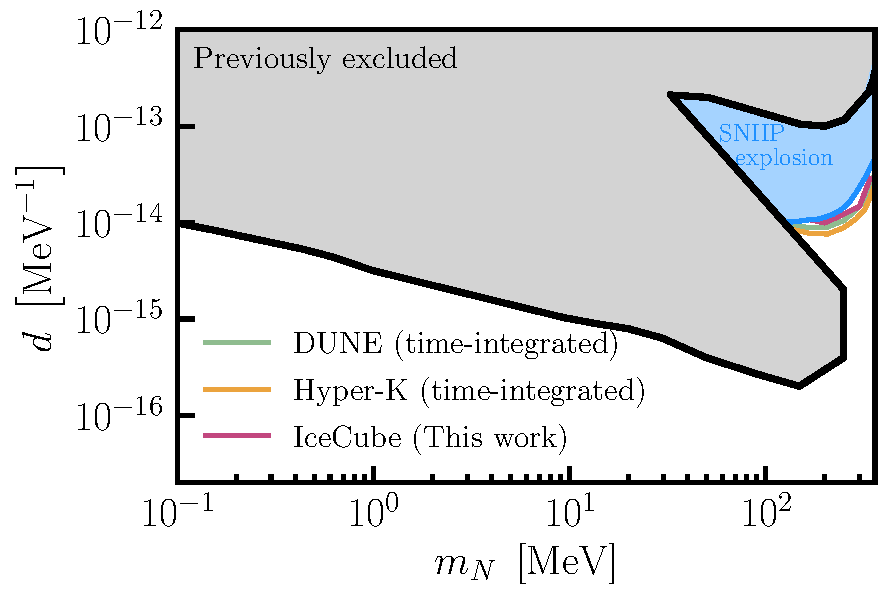
\includegraphics[width=0.47\textwidth]{figures/magnetic_moment_sensitivity}
    \caption{\textbf{\textit{Exclusion sensitivities for the magnetic moment case.}}
    The lines on this plot show the exclusion sensitivity for IceCube, and two next-generation neutrino experiments, Hyper-Kamiokande and DUNE. The shaded regions are excluded by the energy loss constraints, non-observation of photon and neutrino signals from SN1987A studied in \cite{Brdar:2023tmi} and by   constraints on the energy release from SN explosion following \cite{PhysRevLett.128.221103}.
    }
    \label{fig:magnetic_moment_sensitivity}
\end{figure}
The first scenario under consideration is active-to-sterile neutrino transition magnetic moment described by \cite{Magill:2018jla,Brdar:2020quo,Brdar:2023tmi}
\begin{align}
    \mathcal{L} \supset \sum_\alpha d_\alpha \bar{N}\sigma_{\mu\nu} \nu^{\alpha} F^{\mu\nu}-\frac{M_N}{2} \bar{N}^c N + \text{h.c.}\,,
    \label{eq:Lag}
\end{align}
where $\nu^{\alpha}$ and $N$ represent active and sterile neutrinos, respectively. Further, $F^{\mu\nu}$ is the field strength tensor of the electromagnetic field and $d_\alpha$ is the dimensionful coefficient of this dimension-5 term and $M_N$ is sterile neutrino mass. We will abbreviate $d_\alpha \equiv d$ given that we assume flavor universal interaction. The dominant production channels for $N$ inside the SN are $\nu e^- \to \nu e^-$ at lower energies and $\nu \gamma \to N$ for larger active neutrino energies. Both processes occur due to the interaction term in \cref{eq:Lag}; after $N$ are produced, they decay to active neutrinos and photons which is again realized through the same term in the Lagrangian, with the decay width for $N\to\nu\gamma$ given by $\Gamma_N = 6d^2 M_N^3/4 \pi$ \cite{Plestid:2020vqf}. We notice that the time delay near the exclusion boundary are typically of $\Delta t \sim \mathcal{O}(1)$sec, which overlaps with the standard burst time scale. We don't expect improvements over DUNE and Hyper-K. 

{\color{red} Check the bg for DUNE and Hyper-K is the atmospheric neutrino bg which should also contribute to our analysis? IceCube sees at}